
\section{Comparison on benchmarks}
In this section we compare linear Dec-ODE with the state-of-the-art methods using conventional benchmarks. 
\subsection{Experiment Setup \label{sec:experimentSetup}}
\label{sec:setup}
\textbf{Datasets.} 
We used five popular real-world datasets %that are 
from various domains: 
{\bf Reddit} is a sequences of social media posts, 
{\bf Stack Overflow (SO)} is a sequences of rewards received from the question-answering platform, 
{\bf MIMIC-II} is a sequences of diagnosis from Intensive Care Unit (ICU) clinical visits, 
{\bf MOOC} is a sequence of user interactions with the online course,
and {\bf Retweet} is also a sequences of social media posts. See Appendix for detailed description of these datasets. 
To obtain the results in a comparable scale, all time points were scaled down with the standard deviation of time gaps, $\{t_i - t_{i-1}\}_{i=1} ^n$, of the training set similar to \cite{bib:MetaTPP}. 

\textbf{Metrics.} 
We used three conventional metrics for the evaluation: 
1) \textit{negative log-likelihood} (NLL) validates the feasibility of the predicted probability density which is calculated via \eqref{eq:obj}, 2) \textit{root mean squared error} (RMSE) measures the reliability of the predicted time points of events,  
3) \textit{accuracy} (ACC) measures the correctness of the mark distribution $f^*(k|t)$. 
For the prediction, the expected value $\mathbb{E}_{f^*} [t]$ was used as the next arrival time of an event, 
and the mark with the highest probability at time $t$, i.e., $\argmax(f^*(k|t))$, was used as the predicted mark.

\textbf{Baseline.} We compared our methods with three state-of-the-art methods: 
Transformer Hawkes Process (THP) \cite{bib:THP}, Intensity-Free Learning (IFL) \cite{bib:ifl}, and Attentive Neural Hawkes Process (ANHP) \cite{bib:ANHP}. 
As THP and ANHP are both transformer-based methods, they  
effectively leverage the entire observed events $\mathcal{H}_{t_{n}}$ for predicting $e_{n+1}$.
IFL directly predicts $f^*(t,k) = f^*(t) f^*(k|t)$ using a log-normal mixture to predict a flexible distribution. 
Since it parameterizes the distribution $f^*(t)$, $\mathbb{E}_{f^*}[t]$ can be obtained in a closed form.
More details about the implementation are in Sec.\ref{sec:baselineImplementation}.

\begin{table}[!t]
\centering
\caption{Comparison with the state of the art methods on 5 popular real-life datasets. Results with \textbf{boldface} and \underline{underline} represent the best and the second-best results, respectively. Following \cite{bib:THP, bib:ANHP} the mean and std are gained by bootstrapping 1000 times.}
\renewcommand{\arraystretch}{1.3}
\small
\scalebox{0.52}[0.52]{

\begin{tabular}{c | c c c c | c | c c c c | c | c c c c | c} 
& \multicolumn{5}{c|}{RMSE} & \multicolumn{5}{c|}{ACC} & \multicolumn{5}{c}{NLL}\\
\cline{2-6} \cline{7-11} \cline{12-16}
&  RMTPP & THP & IFL & ANHP & \textbf{Dec-ODE} & RMTPP & THP & IFL & ANHP & \textbf{Dec-ODE} & RMTPP & THP & IFL & ANHP & \textbf{Dec-ODE}\\ 
\hline
\hline
\multirow{2}{*}{MOOC} & $0.473$ & $0.476$ & $0.501$ & \underline{$0.470$} & $\textbf{0.467}$
                        & $20.98$ & $24.49$ & $\underline{32.30}$ & $31.53$ & $\textbf{42.08}$ 
                        & $-0.315$ & $0.733$ & $\textbf{-2.895}$ & $\underline{-2.632}$ & $-2.289$  \\  [-3pt]
                    & ${(0.012)}$ & $(0.010)$ & ${(0.012)}$ & $\underline{(0.019)}$ & $\textbf{(0.012)}$
                    & $(0.29)$ &${(0.22)}$ & $\underline{(1.30)}$ & $(0.20)$ & $\textbf{(0.44)}$
                    & $(0.031)$ & $(0.047)$ & $\textbf{(0.031)}$ & $(\underline{0.043})$ & ${(0.191)}$ \\[3pt]
\multirow{2}{*}{Reddit} & $\underline{0.953} $ & $6.151$ & $1.040$ & $1.149$ & $\textbf{0.934}$
                        & $29.67$ & $60.72$ & $48.91$ & $\textbf{63.45}$ & $\underline{62.32}$ 
                        & $3.559$ & $2.335$ & $2.188$ & $\textbf{1.203}$ & $\underline{1.367}$ \\[-3pt]
                        & $\underline{(0.016)}$ & $(0.195)$ &  $(0.017)$ & $(0.010)$ & $\textbf{(0.017)}$
                        & $(1.19)$ & $(0.08)$ & $(1.27)$ & $\textbf{(0.16)}$ & $\underline{(0.11)}$ 
                        & $(0.070)$ &$(0.031)$ & $(0.088)$ & $\textbf{(0.068)}$ & $\underline{(0.126)}$ \\[3pt]
\multirow{2}{*}{Retweet} & $\underline{0.990} $ & $1.055$ & $1.012$ & $1.663$ & $\textbf{0.985}$ 
                        & $51.72$ & $\textbf{60.68} $ & $55.35$ & ${59.72}$ & $\underline{60.17}$ 
                        & $-2.180$ & $-2.597$ & $-2.672$ & $\textbf{-3.134}$ & $\underline{-2.897}$ \\[-3pt]
                    & $\underline{(0.016)}$ & $(0.015)$ & $(0.018)$ & $(0.014)$ & $\textbf{(0.016)}$
                    & $(0.33)$ & $\textbf{(0.11)}$ & $(0.19)$ & $(0.11)$ & $\underline{(0.23)}$ 
                    & $(0.025)$ & $(0.016)$ & $(0.023)$ & $\textbf{(0.019)}$ & $\underline{(0.030)}$ \\[3pt]
\multirow{2}{*}{MIMIC-II} & $\underline{0.859} $ & $>10$ & $1.005$ & $0.933$ & $\textbf{0.810}$ 
                        & $78.20$ & $\textbf{85.98} $ & $80.49$ & $84.30$ & $\underline{85.06}$ 
                        & $1.167$ & $5.657$ & $\textbf{0.939} $ & $\underline{1.025}$ & $1.354$ \\  [-3pt]
                    & $\underline{(0.093)} $ & $(0.114)$ & $(0.121)$ & $(0.088)$ & $\textbf{(0.173)}$
                    & $(5.00)$ & $\textbf{(2.56)} $ & $(5.20)$ & $(2.78)$ & $\underline{(3.65)}$ 
                    & $(0.150)$ & $(0.304)$ & $\textbf{(0.139)} $ & $\underline{(0.155)}$ & $(0.413)$ \\[3pt]
\multirow{2}{*}{} \text{Stack} & $\textbf{1.017} $ & $1.057$ & $1.340$ & $1.052$ & $\underline{1.018}$
                    & $53.95$ & $53.83$ & $53.00$ & $\textbf{56.80}$ & $\underline{55.58}$ 
                    & $2.156$ &$2.318$ & $2.314$ & $\textbf{1.873}$ & $\underline{2.063}$  \\ [-3pt]
                    \text{Overflow} &  $\textbf{(0.011)}$ & $(0.011)$ & $(0.013)$ & $(0.011)$ & $\underline{(0.011)}$
                    & $(0.32)$ & $(0.18)$ & $(0.35)$ & $\textbf{(0.18)} $ & $\underline{(0.29)}$ 
                    & $(0.022)$ & $(0.022)$ & $(0.020)$ & $\textbf{(0.017)} $ & $\underline{(0.016)}$     \\[3pt]
                    \hline
\end{tabular}}
\label{table: real-life}
\end{table}

\subsection{Comparisons of Results}
\label{sec: real-life}

We compare our linear Dec-ODE with state-of-the-art TPP methods on five real-life datasets from Sec. \ref{sec:setup}. The summary of the overall results is in Table \ref{table: real-life}.
In most cases, our approach showed comparable or better results in all metrics. 
It confirms that Dec-ODE successfully models the complex dynamics of MTPP with independently propagated influence functions.
Specifically, Dec-ODE showed its strength in prediction tasks, represented by high accuracy and low RMSE, while ANHP was marginally better in NLL. Moreover, methods that estimate $f^*(t)$ in order to calculate $\mathbb{E}[t]$, Dec-ODE and IFL, showed a tendency to make more accurate predictions of event time.

\textbf{Discussion.} For a fair comparison, we increased the number of sampling used in the thinning algorithm \cite{lec:thinning, bib:thinning_ogata} implemented by \cite{bib:ANHP}. In most cases,the number of samples is multiplied by 20. However, when applied to THP on Reddit dataset the thinning algorithm was not able to correctly sample from $f^*(t)$, since it was not able to correctly sample from an intensity function with low magnitude with high fluctuation.
Details are in Appendix\ref{appen: thinning}.

\subsection{Explainability of Dec-ODE\label{exp: explainability}}

In the case of MTPP and TPP, events temporally and complexly influence $\lambda ^*(t)$ and $f^*(t)$ \cite{bib:hawkesOrigin, ISHAM1979335}. 
Therefore, when considering the explainability of a neural network modeling an MTPP, 
it is important to understand how each event affects the prediction, and how they change through time.
Dec-ODE naturally yields such information. 
For example, the temporal dynamics of $\lambda_g ^* (t)$ and $\hat{f}^*(k|t)$ can be directly observed with the naked eyes as in Fig.  \ref{fig: so fk}.

\begin{wrapfigure}{r}{0.42\textwidth}
% \vspace{-20pt}
    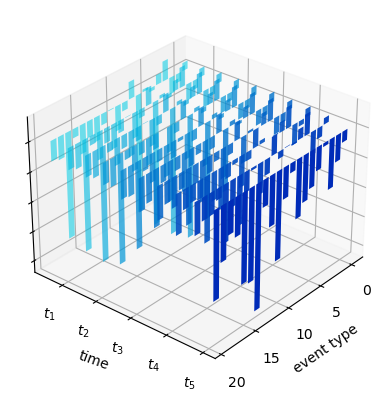
\includegraphics[width=0.92\linewidth, height = 5cm]{figure/fk_dynamic.png}
    \captionsetup[figure]{font=small, justification=justified, margin=0.1cm}
    % \vspace{-10pt}
    \captionof{figure}{Visualization of propagated $\hat{f}^*(k|t, e_i)$ in StackOverflow experiment. The each axis represent time, event type, and the magnitude. 
    The change of influence through time can be easily observed.
    }
    % \vspace{-10pt}
    \label{fig: so fk}
\end{wrapfigure} 

Our detailed investigation on the Retweet dataset further validates the explainability of Dec-ODE. 
For example, some meaningful patterns from the Retweet data is visualized in Fig. \ref{fig:retweet pattern}.
The Retweet data is composed of three classes: 
a post from a person with a small number of followers ($\sim50\%$ of the population),
a post from a person with a medium number of followers$(\sim45\%$ of the population), 
and a post from a person with a large number of followers $(\sim5\%$ of the population), denoted as 0, 1, and 2, respectively.
In Fig. \ref{fig:retweet_inten}, which visualizes $\mu(t;e_i)$ conditioned on different $e_i$, shows that each event exhibits temporally-decaying influence on $\lambda_g(t)$.
Such a pattern is expected as a post on social media shows immediate reactions, rather than a time-delayed effect.
Also, a post from an user with large followers exhibits slower decay.
Which is natural since a post from an user with a large followers gets more exposure and results in longer lasting influence on people.


\begin{figure}
    \centering
    \subfigure[Influence function $\mu(t)$ conditioned on different event types plotted on the same time range.]{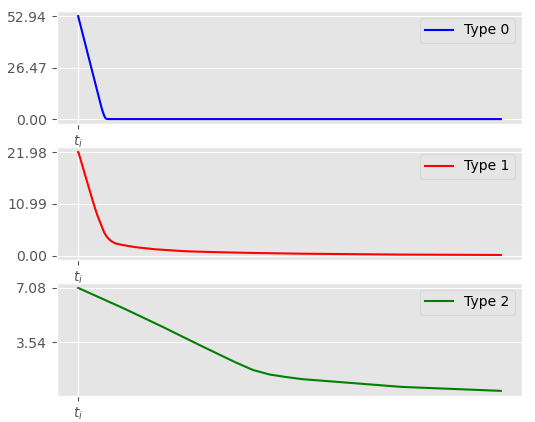
\includegraphics[width = 0.46\linewidth, height = 50mm]{figure/retweet_int.png} \label{fig:retweet_inten}} \hspace{5mm}
    \subfigure[Averaged proportion of influence from different marks on specific marks.]{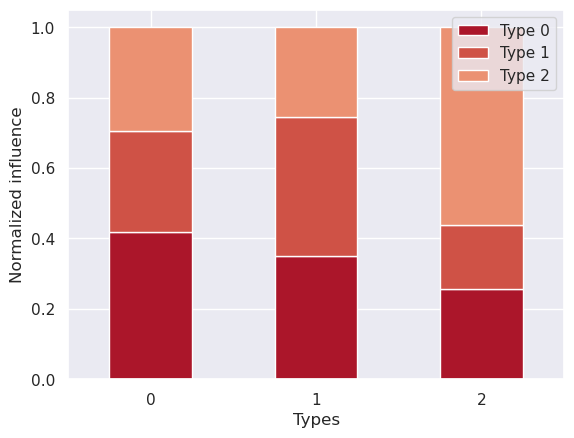
\includegraphics[width=0.46\linewidth, height = 50mm]{figure/retweet_bar.png} \label{fig:retweet_bar}}
    \subfigure[Visualization of events, i.e., marks across time, affecting each other. Blue(0): users with small followers, Red(1): users with medium followers, Green(2): users with large followers. ]{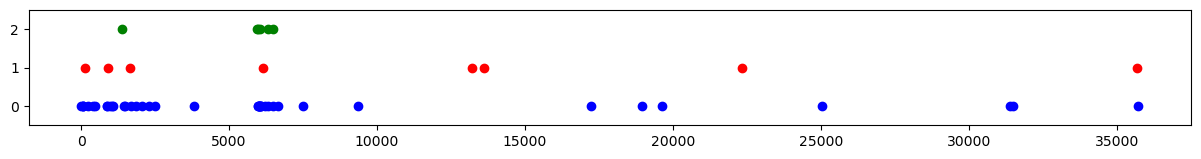
\includegraphics[width = 0.95\linewidth]{figure/retweet_dot.png}\label{fig:retweet_dot}}
    \caption{\small Visualization of patterns found in Retweet dataset. (a) $\mu(t;e_i)$ with different marks, (b) Influence of marks on each other, (c) Actual event marks with respect to time. 
    } 
    \label{fig:retweet pattern}
    % \vspace{-10pt}
\end{figure} 

Moreover, the averaged proportion of influences on different mark types are illustrated in Fig. \ref{fig:retweet_bar}.
First, even though the type 2 takes only $5\%$ of the entire population, it shows great influence in the overall occurrence of events. %This again aligns %with our %common knowledge 
This may be true as a person with many followers may have a greater influence on a broader audience. 
Second, for each event, events with the same types have the strongest influence on each other.
Considering the exponentially decaying patterns of $\mu(t)$ and the large initial magnitude of influence of type 0 shown in Fig. \ref{fig:retweet_inten}, we can infer that events with type 0 would show a high clustering effect 
and actual visualization of the data in Fig. \ref{fig:retweet_dot} validates our reasoning.


% \vspace{-5pt}
\subsection{Parallel Computing Scheme \label{ablation: parallel}}
% \vspace{-5pt}
While Neural ODEs are effective when learning the continuous dynamics of a system, the hidden state propagation requires large computation to solve IVP step by step. 
In Sec. \ref{train_parallel} we proposed to propagate the hidden state through time in parallel by disentangling individual events, 
and we validate the optimization scheme by comparing the average time for each iteration with traditional IVP. 
For the sequential propagation, a differential equation is solved from $t_0$ through $t_n$ step by step.
Table \ref{tab:parallel} summarizes the result, where the computation time significantly decreased in all cases.
Parallel computation for Dec-ODE was at least twice (for MIMIC-II) and as much as five times faster (for Reddit) than the traditional sequential computing scheme. 

\begin{table}[h]
\renewcommand{\arraystretch}{1.1}
\centering
\caption{Training efficiency comparison in different datasets with the average time taken for an iteration (sec/iter) as the metric. Ratio shows that the iteration time at least reduces in half.}
% \vspace{-8pt}
\scalebox{0.57}[0.57]{
\begin{tabular}{cc |c| cc|c | c c|c | cc|c } 
\multicolumn{3}{c|}{StackOverflow} & \multicolumn{3}{c|}{MIMIC-II} & \multicolumn{3}{c|}{Retweet} & \multicolumn{3}{c}{Reddit}\\[-2pt]
\hline
parallel &Sequential& Ratio &  parallel& Sequential&Ratio &  parallel&Sequential&Ratio &  parallel&Sequential&Ratio\\
\hline
\multirow{1}{*}{} $15.0$ & $57.7$ &0.26 & $2.9$ & $6.5$ & $0.47$ & $16.8$ & $67.6$ &$0.25$ & $15.5$ & $78.7$ & $0.20$ \\
   
\end{tabular}
}
\label{tab:parallel}
\end{table}




\section{Linear vs. Non-Linear Influence Function\label{lin-nonlin}}
In the table \ref{table: real-life}, the simple Dec-ODE with linear $\Phi_\lambda$ has been tested.
However, $\Phi_\lambda$ and $\Phi_k$ can be any functions, even neural networks, that satisfy the conditions mentioned in \ref{sec:ground int} and \ref{sec:fk}.
In fact, with linear $\Phi_\lambda$ every influence function must satisfy $\mu(t) \ge 0$ to keep the intensity positive.
Therefore, only an excitatory effect, where an event can only increase the intensity, can be expressed.

In this section, to navigate the extensibility of our framework, a less constrained variant is introduced and tested, denoted as \textit{non-linear} $\Phi_\lambda$. 
The non-linear $\Phi_\lambda(t)$ is defined as follows:
\begin{align}
    \Phi_\lambda(\mu(t;e_0), \cdots, \mu(t;e_i)) = \text{softplus} \bigg( \sum _{e_i \in \mathcal{H}_{t}}  \mu  (t; e_i) \bigg).
\end{align}
Through this modeling approach, an inhibitory effect, where an event decreases the overall intensity, can occur. 

To see how this relaxation affects in modeling TPP, both are tested in a simplified setting, where only the first 40 events of each sequence are used. The results of the experiment are summarized in Table \ref{tab:nonlin} using NLL as the metric. 
The overall result regarding the ground intensity was improved in most situations showing that the intensity function with higher fidelity can be predicted using more flexible $\Phi_\lambda$.

However, non-linear Dec-ODE shows some limitations in predicting a time-delaying effect, where an event does not have a large influence until a certain time passes rather than having an instant influence.
This happens because the inhibitory effect exceeds the excitatory effect, and the intensity function becomes $0$.
In such cases, the inhibitory effect rather impairs the model's ability.
In conclusion, this experiment suggests that with a more flexible $\Phi_\lambda$, prediction can be made with higher fidelity in most cases.
However, adding constraints has to be further discussed to robustly model different patterns in TPP.

\begin{table}[h]
\centering
\caption{Experiment on non-linear $\Phi_\lambda$. The softplus is applied after the summation in order to express inhibitory effects.}
\scalebox{0.9}[0.9]{
\begin{tabular}{cc | cc| c c | cc } \Xhline{0.3ex}
\multicolumn{2}{c|}{StackOverflow} & \multicolumn{2}{c|}{MIMIC-II} & \multicolumn{2}{c|}{Retweet} & \multicolumn{2}{c}{Reddit}\\[-2pt]
Linear & Non-linear &  Linear & Non-linear  &  Linear & Non-linear  & Linear & Non-linear\\
\hline
\multirow{1}{*}{} $0.9948$ & $\textbf{0.8987}$ &0.2451 & $\textbf{0.2183}$ & $-5.0872$ & $\textbf{-5.1649}$ & $\textbf{0.5163}$ & $18.2571$ \\
\Xhline{0.3ex}      
\end{tabular}}
    \label{tab:nonlin}
\end{table}

\section{Imputation \label{appen:imputation}}

In this section, we investigate the effect of independently modeling hidden state dynamics by comparing it with methods using contextual information.
Events from the StackOverflow dataset are randomly dropped to see how the behavior changes as the number of observed events decreases. 

\setlength{\intextsep}{0pt}
\begin{wrapfigure}{r}{0.46\textwidth}
    \centering
    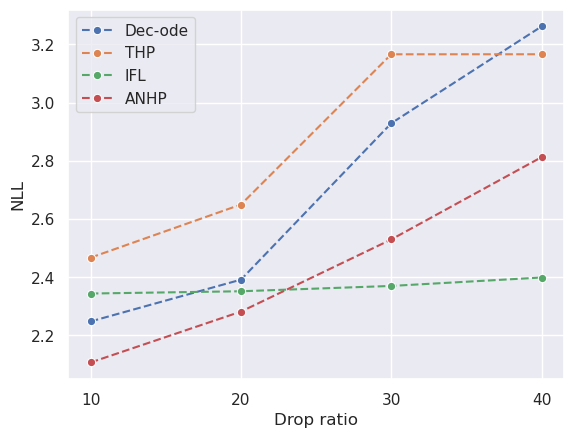
\includegraphics[width=0.44\textwidth]{figure/imputation.png}
    \caption{\raggedright Imputation experiment done using Stackoverflow dataset, where from $10\%$ to $40\%$ of data are randomly dropped.}  
    \label{fig:imputation}
\end{wrapfigure} For the fair comparison, we randomly selected 90\%, 80\%, 70\%, and 60\% indexes from the test dataset, and saved the data with the selected indexes as new test sets.
The results using the new test sets are visualized in figure \ref{fig:imputation}.
The graph illustrates that the decrease in performance of Dec-ODEs shows a similar tendency when compared to others.

The result suggests that other methods cannot retrieve the loss of information.
This statement can be made since Dec-ODE, which does not consider inter-event relationships, shows a similar tendency.

\section{Simulation Study}

\begin{table}[h]
    \centering
    \begin{tabular}{c|c|c|c}
            & RMSE   & ACC   & NLL    \\ \hline
    THP     & 0.7734 & 27.48 & 3.0121 \\ 
    ANHP    & 0.6528 & 30.31 & 0.2807 \\ 
    Dec-ODE & \textbf{0.6568} & \textbf{30.35} & \textbf{0.2739} 
    \end{tabular}
    \caption{Estimation accuracy on the simulated Hawkes process. }
        \label{tab:simulation}
    \end{table}

We have performed a simulation study on the Hawkes process following a similar procedure from the Neural Hawkes Process (NHP) \cite{bib:nhp}. 
In order to obtain the true intensity function we randomly sampled the parameters for the kernel function of the multivariate Hawkes process, and we simulated synthetic data using the tick library \cite{bacry2018tick}. 
The range of the sampling was changed from the NHP since the scale in the library was different from the paper.
In Figure \ref{fig:sim_a} - \ref{fig:sim_d}, THP struggles to simulate the flexible dynamics of the intensity function $\lambda_g$, whereas ANHP and Dec-ODE show similar dynamics to the ground truth intensity. 
The table \ref{tab:simulation} also demonstrates that Dec-ODE shows better results than THP and ANHP in all metrics. 
The result also aligns with the results in Table \ref{table: real-life}, which suggests that Dec-ODE can simulate reliable MTPPs compared to other state-of-the-art methods. 
Figure \ref{fig:sim_ae} illustrates $\mu(t)$ that compose $\lambda_g(t)$ from Figure \ref{fig:sim_d}, which shows that the ground intensity $\lambda_g(t)$ can be reconstructed from the individually constructed trajectory, i.e. an MTPP can be modeled from decoupled information.

\begin{figure}[h]
    \centering
    \subfigure[]{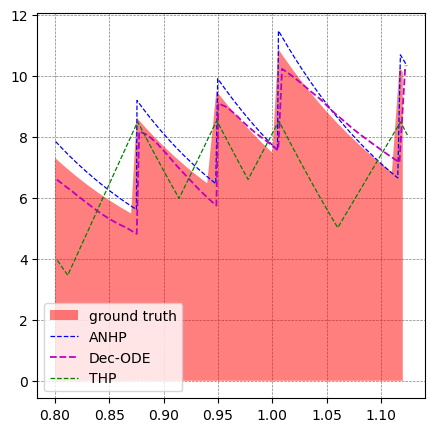
\includegraphics[height = 0.3\linewidth]{figure/total_intensity1.png}\label{fig:sim_a}}\hspace{-1mm}
    \subfigure[]{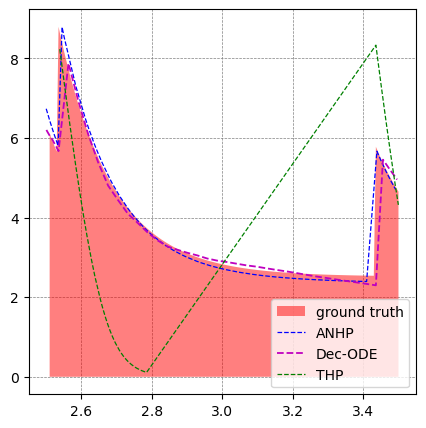
\includegraphics[height = 0.3\linewidth]{figure/total_intensity2.png}\label{fig:sim_b}}\hspace{-1mm}
    \subfigure[]{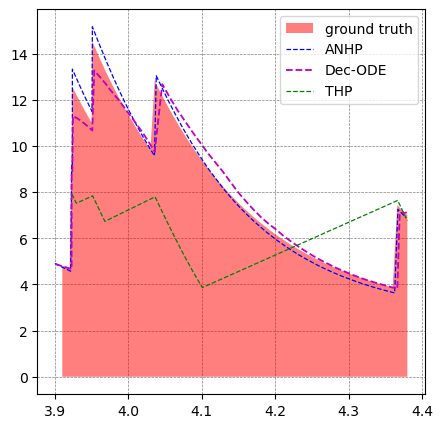
\includegraphics[height = 0.3\linewidth]{figure/total_intensity3.png}\label{fig:sim_c}}\hspace{-1mm}
    \subfigure[]{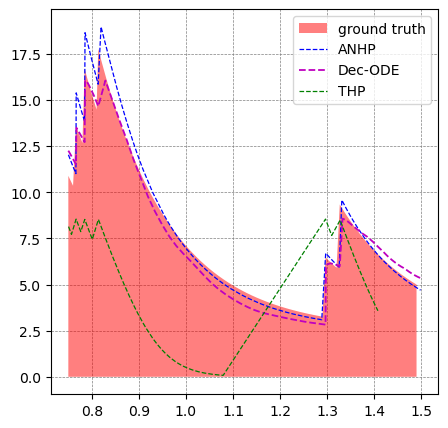
\includegraphics[height = 0.35\linewidth]{figure/total_intensity4.png}\label{fig:sim_d}}\hspace{1mm}
    \subfigure[]{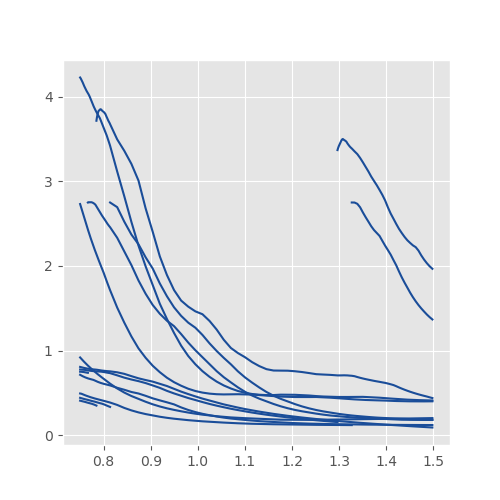
\includegraphics[height = 0.4\linewidth]{figure/decoupled_intensity4.png}\label{fig:sim_ae}}\hspace{1mm}
    \caption{Visualization from a simulation study. (a), (b), (c), and (d) compare the true intensity function of a Hawkes process and the reconstructed results from THP, ANHP, and Dec-ODEs. Each $\mu(t)$ that composes the result in (d) is illustrated in (e).}
    \label{fig:simulation}
\end{figure}



\section{Train time comparison}

In order to compare the time required for training, the time required for training one epoch (sec / epoch) is measured. The experiment is conducted on a single NVIDIA RTX A6000 GPU (48GB) with the largest batch size possible for the GPU. The result can be found in the table \ref{tab:epoch_time}. THP required the least amount of time, while methods predicting intensity at each time point showed a relatively slower training rate. In most cases, Dec-ODE shows a shorter training time per epoch.
\begin{table}[h]
    \renewcommand{\arraystretch}{1.1}
    \centering
    \caption{Training time (sec / epoch) compared between THP, ANHP, and Dec-ODE.}
    % \vspace{-8pt}
    \scalebox{0.9}[0.9]{
    \begin{tabular}{c| c| c | c | c | c } \Xhline{0.3ex}
    & \multicolumn{1}{c|}{MOOC} & \multicolumn{1}{c|}{Reddit} & \multicolumn{1}{c|}{Retweet} & \multicolumn{1}{c|}{Stackoverflow} & \multicolumn{1}{c}{MIMIC-II}\\[-2pt]
    \hline
    THP & $12.94$ & $66.95$ & $34.05$ & $13.36$ & $2.27$ \\
    ANHP & $835.36$ & $541.20$ & $630.64$ &$129.51$ & $3.69$ \\
    Dec-ODE & $117.35$ & $242.75$ & $484.08$ & $123.28$ & $8.12$\\
        
    \Xhline{0.3ex}      
    \end{tabular}
    }
        \label{tab:epoch_time}
    
    \end{table}
    
    \begin{table}[h]
    \renewcommand{\arraystretch}{1.1}
    \centering
    \caption{Required memory (MB) compared between baseline methods with batch size 4.}
    
    \scalebox{0.8}[0.8]{
    \begin{tabular}{c| c| c | c | c | c } \Xhline{0.3ex}
    & \multicolumn{1}{c|}{MOOC} & \multicolumn{1}{c|}{Reddit} & \multicolumn{1}{c|}{Retweet} & \multicolumn{1}{c|}{Stackoverflow} & \multicolumn{1}{c}{MIMIC-II}\\[-2pt]
    \hline
    RMTPP & $1110 + 1114$ & $1706 + 1142$ & $1294 + 1112$ & $1306 + 1114$ & $1114 + 1106$ \\
    THP & $3484$ & $15304$ & $1678$ & $3808$ & $1130$ \\
    ANHP & $31310$ & $< 48$ GB & $11790$ &$39260$ & $1244$ \\
    Dec-ODE & $1422$ & $1472$ & $1314$ & $1422$ & $1470$\\
    \Xhline{0.3ex}      
    \end{tabular}
    }
        \label{tab:epoch_memory}
    \end{table}
\section{Implementation details}

\subsection{IVP solving with varying time intervals \label{appen: varied time}} 
Initial Value Problem (IVP) solving with varying time intervals is done following the method introduced in \cite{bib:STPP}.
In short, the integration in the region $[t_{start}, t_{end}]$ is solved within $[0, 1]$ and scaled back to the original region. 
Using this method, every time interval with different lengths can be computed within the same number of steps.
We apply this for both batch computations with different lengths and parallel computation of $h(t;e_i)$ in Sec. \ref{train_parallel}.

\subsection{Batch Computation}
Our method propagates $h(t)$  further than $t_N$, which is the last observed point.
Therefore, in order to cover the full range of $f^*(t)$, two different masking operations are required.
The first one is the one commonly used when dealing with sequences with different lengths, and we call it the \textit{sequence mask}.
With sequences with different lengths, unobserved events should be ignored for both training and inference, and the sequence mask is used to ignore unobserved time points.
The second mask is the \textit{propagation mask}, where the unobserved time points after $t_N$ are not masked.
This is used for solving ODEs to propagate $h(t)$ until the decoded $\mu(t)$ converges.


\subsection{Baseline \label{sec:baselineImplementation}}

For THP and ANHP, we used the public GitHub \href{https://github.com/yangalan123/anhp-andtt}{repository} (\cite{bib:ANHP} with MIT License).
The code for the THP has been modified by \cite{bib:ANHP}, where time and event prediction is now made by using $\lambda(t)$ with a thinning algorithm instead of the prediction module that is parameterized by neural networks.

Moreover, as mentioned in the public GitHub repository of THP, there is an error regarding the NLL computation. In both published versions, NLL is computed conditioned on the observed history information and a current event. i.e., $L(e_i) = f(e_i|e_0, \cdots, e_i)$. Therefore, the calculation of the intensity has been corrected to $L(e_i) = f(e_i|e_0, \cdots, e_{i-1})$, where the modification is made based on the code used for the integration.

For IFL, we used the public GitHub repository \href{https://github.com/shchur/ifl-tpp}{https://github.com/shchur/ifl-tpp} (\cite{bib:ifl}, no license specified). Some modifications have been made since the original implementation does not support time point prediction. The modification was made based on the author's comment made in the ``issue'' page of the repository. However, the computation of $\mathbb{E}[t]$ was not stable due to the high variance of components in the mixture model. In other words, when a distribution in a mixture model has a high variance, the exponential term in the calculation causes an overflow, which leads to an overflow of the entire calculation. 
Therefore, we have tightened the parameters for the gradient clipping in \cite{bib:ifl}, as done in \cite{bib:MetaTPP}.


\subsection{Thinning algorithm\label{appen: thinning}}
For the experiment done in Table \ref{table: real-life}, we tested different parameters for the thinning algorithm \cite{lec:thinning, bib:thinning_ogata}, implemented by \cite{bib:ANHP}, for a fair comparison.
THP and ANHP sample the next time points using the thinning algorithm then take their average to compute $\mathbf{E}[t]$.

The thinning algorithm resembles the rejection sampling, in which the proposal is accepted with the probability $\lambda(t) / \lambda_{up}$ where $\lambda_{up} \geq \lambda(t)$ for all $t\in(t_{i-1}, \infty)$ \cite{bib:nhp}.
Therefore, reliable $\lambda_{up}$ is required to sample from the correct distribution.
If $\lambda_{up}$ is too high, all the samples would be rejected, whereas accept incorrect samples if $\lambda_{up}$ is too low.

In the implementation, $\lambda_{up}$ is calculated by $c * max(\lambda(s_0), \cdots, (s_m))$, where $c$ is a constant, $m$ is the number of samples used for the calculation, and $s_m$ is a uniformly sampled time point.
To find correct $\lambda_{up}$, for most of the reported results in Table \ref{table: real-life}, we increased the number of $m$ by $\times10$.
When overall $\lambda(t)$ is too low, the scale goes up to $1000$ in the most extreme case.

\subsection{Training Details}
When tuning the simple Dec-ODE, three different hyperparameters are considered for the model structure with the addition of an Initial Value Problem (IVP) solving method.
Three hyperparameters are the dimension of hidden state $D$, the dimension of linear layers of neural networks $N$, and the number of liner layers $L$.
We haven't fully searched for the optimal parameters for each dataset. For testing, we rather applied similar parameters to all datasets.

Throughout the experiment, $D$ was chosen from $\{32, 64\}$. However, since the dynamics of $h(t)$ is highly dependent on the information in the hidden state, we expect a higher dimension would enable the neural network to learn more difficult dynamics.

The width of linear layers $N$ is chosen between $\{128, 256\}$, and the number of layers are tested between $\{3, 4, 5\}$. In most cases, the number of layers did not show much improvement in the results.

The three hyperparameters above that showed the best result are chosen. However, in most cases, $D=64$, $N=256$, and $L=3$ were used.

In the case of IVP solver, two different methods were used training and testing. For training, Euler's method was used in most cases for efficiency. The purpose of training is to learn the dynamics of hidden state $h(t)$, and we believe Euler's method sufficiently satisfies such purpose, and we haven't thoroughly looked into the benefits of using different solvers.

During testing $\lambda_g(t)$, to make a more precise approximation, we utilize Runge-Kutta method with fixed step size, generally referred to as RK4. The computation of RK4 method is as follows:
\begin{align}
    y_{n+1} &= y_n + {h\over6}(k_1 + 2k_2 + 2k_3 + k_4)\\
    t_{n+1} &= t_n + h
\end{align}
where,
\begin{align}
k_1 &= f(t_n, y_n), \\
k_2 &= f(t_n + {h \over 2}, y_n + h {k_1 \over 2}),\\
k_3 &= f(t_n + {h \over 2}, y_n + h {k_2 \over 2}),\\
k_4 &= f(t_n + h, y_n + hk_3).
\end{align}

The RK4 method can more precisely model the trajectory compared to Euler's method. 
Therefore, there is less error in the estimated $f^*(t)$.
Other methods such as dopri5, RK4 with step size control, and other variants of IVP solvers can be applied for more accurate results.

To solve the IVP, we fixed the number of steps required for solving from $t_i$ to $t_{i+1}$. Similar to the IVP solver, we used a simpler setting for the training and a more precise setting for the testing. During training, in most cases, we used 16 steps in between every event. The increase in number is expected to improve the result, yet we have not thoroughly looked into it since it shows comparable results with state-of-the-art methods. During testing, we increased the number to 64.

When testing $f(k|t)$, the precise approximation of $\hat{f} (k|t, e_i)$ did not show a visible effect on the result.
Therefore, for computational efficiency, Euler's method was used with the same number of step sizes used for training.



\section{Dataset Description}
\begin{table}[h]
    \centering
    \renewcommand{\arraystretch}{1.3}
        \begin{tabular}{c|c c c c}
            Datasets & \# of Seq. & \# of Events & Max Seq. Length & \# of Marks \\
            \hline
             MOOC & 7,047 & 389,407 & 200 & 97 \\ 
             Reddit & 10,000 & 532,026 & 100 & 984 \\ 
             Retweet & 24,000 & 21173,533 & 264 & 3 \\ 
             StackOverflow & 6,633 & 480,414 & 736 & 22 \\ 
             MIMIC-II & 650 & 2419 & 33 & 75 \\ 
        \end{tabular}
        \caption{Statistics of benchmark datasets used for comparisons.}
        \label{tab:data_stat}
    \end{table}
% Table \ref{tab:data_stat} shows the statistics of each benchmark dataset used for testing.

\subsection{Benchmark dataset}
MIMIC-II and Retweet were from the public GitHub repository \href{https://github.com/SimiaoZuo/Transformer-Hawkes-Process} (\cite{bib:THP}, with no license specified). Others were also from the public GihtHub repository \href{https://github.com/BIRD-TAO/GNTPP} (\cite{bib:exploring_generative}, with no license specified). 

\subsection{Data preprocess}
When dealing with Mooc, Reddit, Retweet, and StackOverflow, two modifications to the dataset have been made.
First, when two events have the same time point, one of the events is removed.
We chose the latter one in the dataset.
This is because when $t_i - t_{i-1} = 0$, IFL was not able to properly estimate $f^*(t)$.
Also, in many cases, TPP assumes 2 or more events happening at the same time as improbable.
Second, as mentioned in Sec. \ref{sec:experimentSetup}, data were scaled by the standard deviation of $\{t_{i} - t_{i-1}\}_{i=0} ^n$.
When the scale of $t_i - t_{i-1}$ is too large, overflow happens during the calculations.
Therefore, we tried to make the scale similar to the results from \cite{bib:MetaTPP}, but the standard deviation was chosen since the scale was not specified in the published work.


\section{Visualizations}

From the figures, we can identify that each data show difference in dynamics. 
For instance, in $\mu(t;e_i)$ we can identify that each influence shows a delaying effect where the effect of an event affects others after some time passes.

% \subsection{Vector field}
% By employing Neural ODEs \cite{bib:node} we can visualize the overall dynamics of functions that we estimate.
% Fig. \ref{fig:vectorfields} visualizes the vector fields.
% Fig. \ref{fig:hstateVector} visualizes the first dimension of the hidden state using the StackOverflow dataset.
% The arrow represents the dynamics where the value of the tail is given as the input.
% There are some visible patterns in the dynamic forms.
% However, a certain part of the field shows very different behavior even when they receive the same input.
% It shows that the hidden state dynamics learned from the data is very complex.
% On the other hand, $\mu(t;e_i)$ visualized in Fig. \ref{fig:muVector} shows a clear tendency in the region.

% \begin{figure}[b]
%     \centering
%     \subfigure[Visualization of the hidden state dynamics with StackOverflow dataset.]{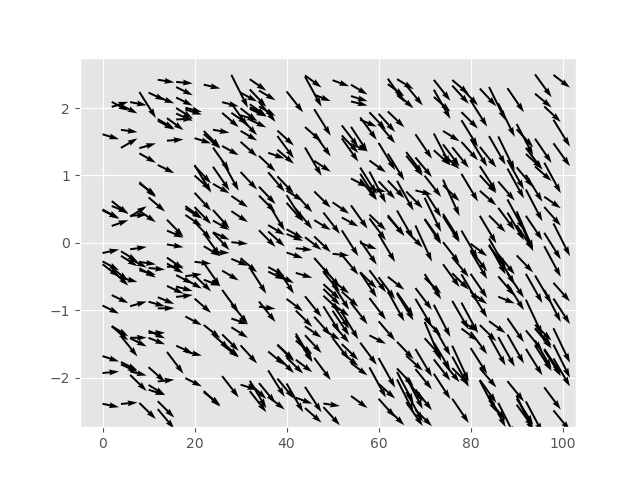
\includegraphics[width=0.45\linewidth]{figure/hs_dynamic2.png}\label{fig:hstateVector}}\hspace{5mm}
%     \subfigure[Visualization of the change of $\mu(t;e_i)$ in StackOverflow dataset. ]{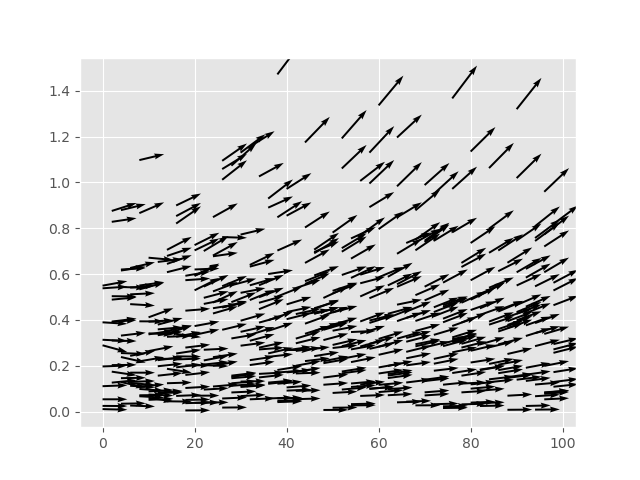
\includegraphics[width=0.45\linewidth]{figure/intensity_dynamic.png}\label{fig:muVector}}
%     \caption{Visualization of vector fields. a) is a vector field of the hidden state and b) is the vector field of $\mu(t;e_i)$. The length of the arrow represents the magnitude.}
%     \label{fig:vectorfields}
% \end{figure}
% % \vspace*{3in}

% \subsection{Visualization of Continuous Dynamics}
\begin{figure}[hb]
    % \setlength{\subfigtopskip}{0pt}   % Removes space between image and caption
    % \setlength{\subfigbottomskip}{0pt} % Removes space below the caption

    \centering
    \subfigure[Visualization of $\mu(t;e_i)$ trained using MOOC.]
    {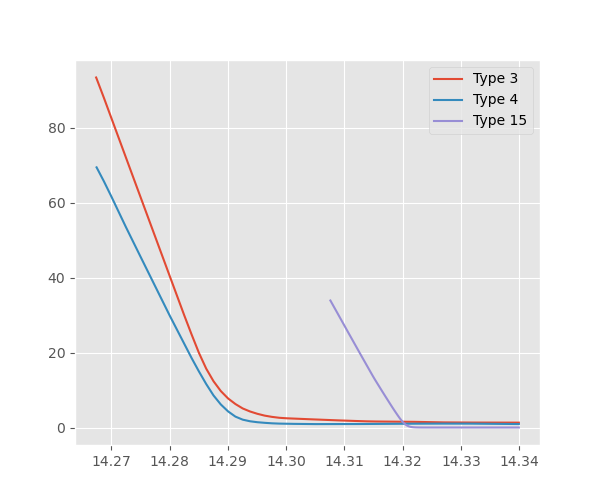
\includegraphics[height = 0.4\textwidth]{figure/mooc_inten.png}}
    \hfill
    \subfigure[\raggedright $\hat{f}(t;e_{i})$ trained using in MOOC.]
    {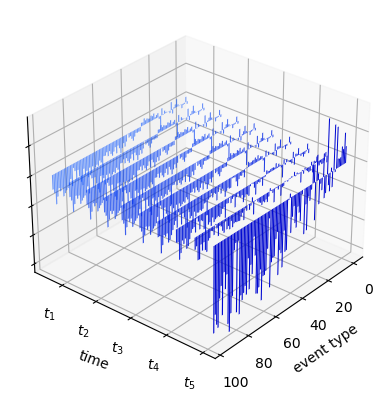
\includegraphics[height = 0.4\textwidth]
    {figure/mook_fk_14.png}}
    \caption{Visualization of dynamics of $\mu$ and $\hat{f}$ in benchmark dataset. (a) is a visualization of ground intensity trained on MOOC dataset, and (b) is a visualization of $\hat{f}(t;e_i)$ changing through time trained using MOOC dataset.}
\end{figure}

\begin{figure}[ht] \ContinuedFloat
    % \vspace{-0.3cm}
    \subfigure[$\mu(t;e_i)$ trained using Reddit.]
    {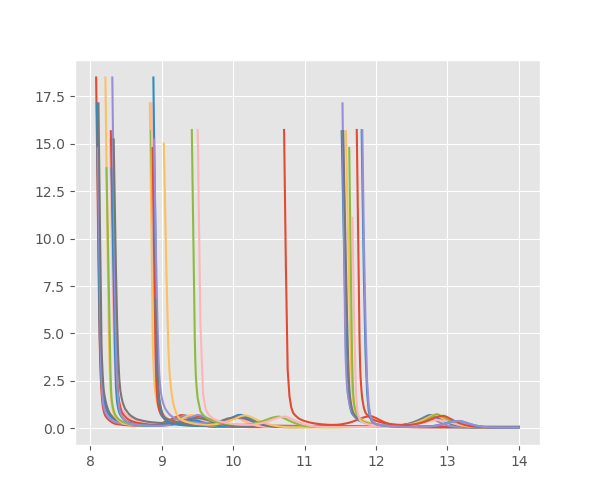
\includegraphics[height = 0.4\textwidth]{figure/reddit_inten.png}}
    \hfill
    \subfigure[\raggedright $\hat{f}(t;e_{i})$ trained on Reddit dataset.]
    {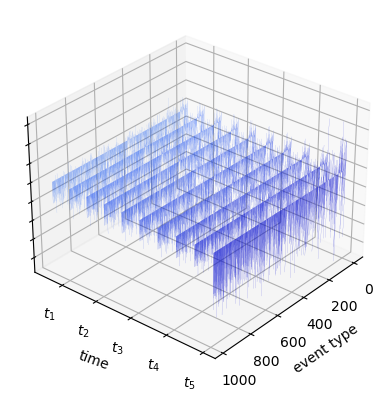
\includegraphics[height = 0.4\textwidth]
    {figure/reddit_fk_148.png}}

    % \vspace{-.3cm}
    \subfigure[Visualization of $\mu(t;e_i)$ trained using SO.]
    {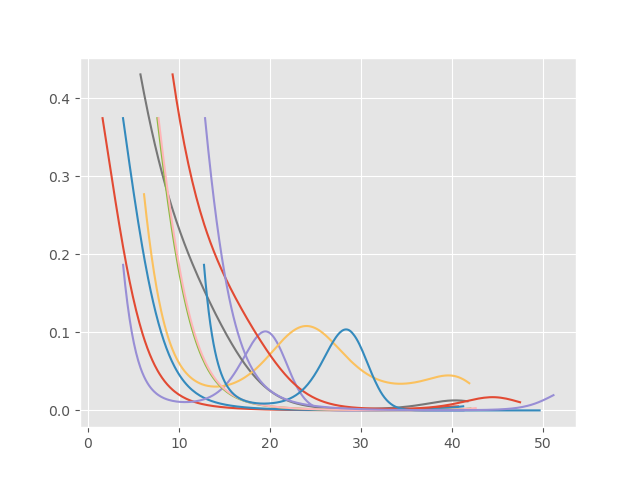
\includegraphics[height = 0.4\textwidth]{figure/SO_int.png}}
    \hfill
    \subfigure[\raggedright Visualization of $\hat{f}(t;e_{i})$ in MIMIC.]
    {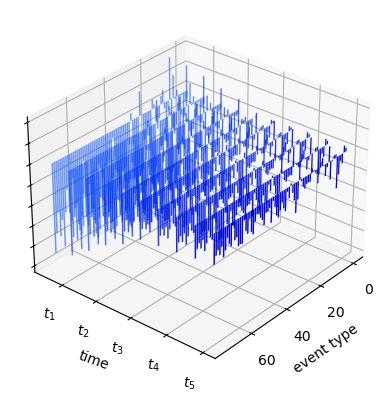
\includegraphics[height = 0.4\textwidth]{figure/mimic_fk_10.png}}
    \caption{Visualization of dynamics of $\mu$ and $\hat{f}$ in benchmark dataset. (a) is a visualization of ground intensity trained on Reddit dataset, (b) is a visualization of $\hat{f}(t;e_i)$ changing through time trained using Reddit dataset, (c) shows dynamics of ground intensity trained using Stack Overflow dataset, and (d) shows $\hat{f}(t; e_i)$ changing through time trained using MIMIC-II dataset.}
    \label{fig:mooc}

\end{figure}

